
%\chapter{Reconstruction of Pt/Pd Bimetallic Near Surface Alloys Exposed to Carbon Monoxide}
\chapter{RECONSTRUCTION OF PT/PD BIMETALLIC NEAR SURFACE ALLOYS EXPOSED TO CARBON MONOXIDE}
\label{app:nsa}

\section{Introduction}


%intro line about catalysts
Catalysts are at the center of numerous industrial and scientific processes;
however many of the most effective catalysts are composed of expensive metals
such as \ce{Pt}, \ce{Pd}, \ce{Rh}, \ce{Au}, and \ce{Ag}.  In order to address
this issue of cost, there has been a push to design and characterize new
bimetallic materials,\citep{Han:2015qr, Yu:2012by} near-surface alloys
(NSA),\citep{Stephens:2011bv, Jan-Knudsen:2007fe} and dispersed
nanostructures\citep{Shibata:2002hh, Kugai:2011rt} from less expensive metals
and other materials.  The goal is for these catalysts to still be highly active
while reducing the cost of the catalyst. This can be done by replacing a
significant amount of the expensive metal with a cheaper one.  As an example
\ce{Pt3Ni} catalysts have been created that show an increased activity for the
oxygen reduction reaction while replacing a portion of \ce{Pt} with the much
cheaper \ce{Ni}.\citep{Tuaev:2013fk, Stamenkovic:2007kk} The stability of these
types of materials is called into question however as Tao {\em et al.} showed
in their study of \ce{Pd/Rh} core-shell nanoparticles, which experienced
large-scale inversions of material depending on the oxidizing or reducing
nature of the environment.\citep{Tao:2008aa} That is, under an oxidizing
atmosphere, \ce{Rh} made up the outer shell of the nanoparticle while under a
reducing atmosphere, \ce{Pd} migrated to the surface instead. This appendix
provides information on the initial creation of bimetallic Pt/Pd near-surface
alloys and the preliminary results obtained.

\section{Methodology}
Two main systems were examined differing only by the displayed surface facet,
(111) or (100).  The (111) systems were initially thermalized at 200~K and
warmed up in the canonical (NVT) ensemble  to 1000~K over 500 ps. They were
then allowed to reach equilibrium at this temperature over another 500 ps at
which point they were dosed with a sufficient quantity of \ce{CO} to correspond
to either 0, 0.25, or 0.5 monolayers (ML) of coverage. The systems were further
equilibrated in the NVT ensemble for another 500 ps before switching to the
microcanonical (NVE) ensemble for 6 ns of data collection. The (100) systems
were treated identically except that they were warmed and equilibrated at 600~K
and kept at that temperature throughout the simulation.

\subsection{Interaction potentials}
The interaction potentials provided in Michalka {\em et
al.}\citep{Michalka:2015aa} are used here unchanged. Important to note is that
the \ce{Pd\bond{-}CO} interaction is slightly more favorable by 0.2 kcal/mole
when compared to the \ce{Pt\bond{-}CO} interaction in this parameterization.

\subsection{System details}
The systems were constructed from a FCC \ce{Pt} crystal that was ``sliced'' to
display either a (111) or (100) facet in the {\em z}-direction while being
periodic in the {\em x} and {\em y} directions. The bulk of the crystal was
kept as \ce{Pt} while one or two layers directly underneath the surface were
converted to \ce{Pd}. The ideal systems, before the addition of \ce{CO}, are
highlighted in the top row of Figure \ref{fig:biSystems}. The (111) systems
have dimensions of $71.41\times82.44\times100$ \AA\textsuperscript{3}, while
the (100) systems have $68.78\times68.78\times100$ \AA\textsuperscript{3}.
Knowing that the \ce{Pd\bond{-}CO} interaction is stronger, it was chosen as
the subsurface layer. Additionally, when \ce{Pt} is on the surface, there are
two effects that could encourage restructuring, \ce{Pt}'s higher cohesive
energy, ({\em i.e.} desire to be in a bulk environment), and the greater
strength of the \ce{Pd\bond{-}CO} compared to the \ce{Pt\bond{-}CO}
interaction.

\begin{table}
  \caption{PT/PD NEAR SURFACE ALLOY SIZES AND COMPOSITION}
  \centering
  \begin{threeparttable}
  \begin{tabular}{ c ccc }
  \hline
  \hline
  \textbf{System} & \textbf{Pt} & \textbf{Pd} &  \textbf{(Pd/total)} \\
  \hline
  100-1Pt-1Pd & 7776 & 1296  & 0.143 \\
  100-1Pt-2Pd & 6480  & 2592  & 0.286 \\
  111-1Pt-1Pd & 10800  & 1800  & 0.143 \\
  111-1Pt-2Pd & 9000 & 3600  & 0.286 \\
  \hline
  \hline
  \end{tabular}
  \end{threeparttable}
\label{tab:systems1}
\end{table}


\begin{landscape}
\begin{figure}[p!]
\centering
  \includegraphics[width=0.8\linewidth]{../figures/appD/systems.pdf}
  \caption{Depictions of the (111) and (100) systems. \ce{Pt} atoms are colored
gray while \ce{Pd} are colored pink. The top row depicts near surface alloys
with a sandwiched Pt (surface), Pd (subsurface), Pt (bulk) system before
significant warming while the bottom row depicts the same systems after six ns of
exposure to CO. Systems (a) and (b) display the low-energy (111) facets and
only differ with number of layers of Pd with (a) having one layer and (b)
having two layers. Systems (c) and (d) display the (100) facets on the surface
and are only different with regard to the number of Pd layers, one and two
respectively.}
\label{fig:biSystems}
\end{figure}
\end{landscape}

\section{Results \& Discussion}
The (100) \ce{Pt} surfaces were unstable at the temperatures
simulated regardless of CO-coverage as the surface \ce{Pt} collapsed to domains
of (111). This had the effect of exposing the underlying (100) \ce{Pd} which
remained stable during the simulation. This change is highlighted in Figures
\ref{fig:biSystems}.c and \ref{fig:biSystems}.d, where the initially (100)
surface restructures to the lower energy (111) domains exposing large patches
of \ce{Pd} to the \ce{CO} in the system. This is shown a bit more clearly in
Figure \ref{fig:surfaceGrid} although a small portion of the surface did retain
the original (100) motif (highlighted in yellow). Additionally, because of the
way adsorbate coverage was initially calculated, this restructuring of the
(100) surface creates more binding sites for the \ce{CO} to bind too which can
be seen by comparing the (111) to the (100) systems in Figure
\ref{fig:biSystems} and seeing the large amount of \ce{CO} that is not adsorbed
in the (111) systems.

\subsection{Inversion}
One mechanism for surface restructuring is that of atom inversion or surface
segregation, where an atom from a subsurface layer exchanges positions with an
atom on the surface.  This process strongly depends on the stability of the
surface and specifically on  the strength of metal-metal interactions as many
of these bonds will need to be broken or weakened for this process to occur.
The \ce{Pt/Pd} systems modeled in this study showed some evidence of this
process over the short amount of simulation time, specifically on the higher
\ce{CO} coverage systems. As highlighted in Figure \ref{fig:inversion}, over a
period of 5 ns (left image 1 ns, right image 6 ns) an additional 6 \ce{Pt}
surface atoms were replaced with the subsurface \ce{Pd}.  This process is
energetically favorable because the \ce{Pt\bond{-}Pt} and \ce{Pt\bond{-}Pd}
bonds are stronger than the \ce{Pd\bond{-}Pd} interactions.  However, the
kinetic barrier for this process is large since it requires some amount of
lifting or compressing of the surface atom as well as a small vacancy formation
at some point in the subsurface. Henkelman {\em et al.} modeling (111) and
(100) \ce{Au/Pd} surfaces observed that the presence of a vacancy on the surface
drastically increased the rates of surface segregation.\citep{Kim:2013mi} The
presence of \ce{CO} appears to slightly lower the barriers needed for this
process as the systems with \ce{CO} were observed to have a greater number of
\ce{Pd} on the surface at the end of the simulations. If the systems had been
run for significantly longer, it is likely that small domains or patches of
\ce{Pd} would have formed on the surface, as the most energetically favored
sites for inversion would be those that already had a \ce{Pd} atom nearby.
While inversion events were observed to occur on the (100) surfaces, the loss
of a complete surface coverage of \ce{Pt} because of the refaceting from (100)
to (111) makes exact characterization of such events difficult.


\begin{figure}[p!]
\centering
\includegraphics[width=\linewidth]{../figures/appD/inversion.pdf}
\caption{Observed inversion events on the 111-1\ce{Pt}-1\ce{Pd} surface with a
0.5 ML coverage of \ce{CO}. The left image (a) is of the surface after one ns
of data collection while the right image (b) is taken at the end of six ns.
\ce{Pd} atoms are shown in pink and \ce{Pt} atoms are shown in gray.}
\label{fig:inversion}
\end{figure}

\subsection{Domain formation}
Using the same methodology as developed in reference \citep{Michalka:2015aa},
the surfaces of the systems were projected onto a two-dimensional grid which
was then digitized and analyzed to collect distributions of domain sizes of
\ce{Pt} and \ce{Pd}. An example of this process is illustrated in Figure
\ref{fig:surfaceGrid}. 
The distribution of domain sizes can then be plotted as a
function of time and \ce{CO} coverage as illustrated in Figures
\ref{fig:ds100Pt} and \ref{fig:ds100Pd}. This analysis was also run on the
(111) systems, and while the presence of inversion events does lead to a number
of ``small'' \ce{Pd} domains, the surfaces remain overwhelming \ce{Pt}, at
least during the performed simulation time.

\begin{landscape}
\begin{figure}[p!]
\centering
  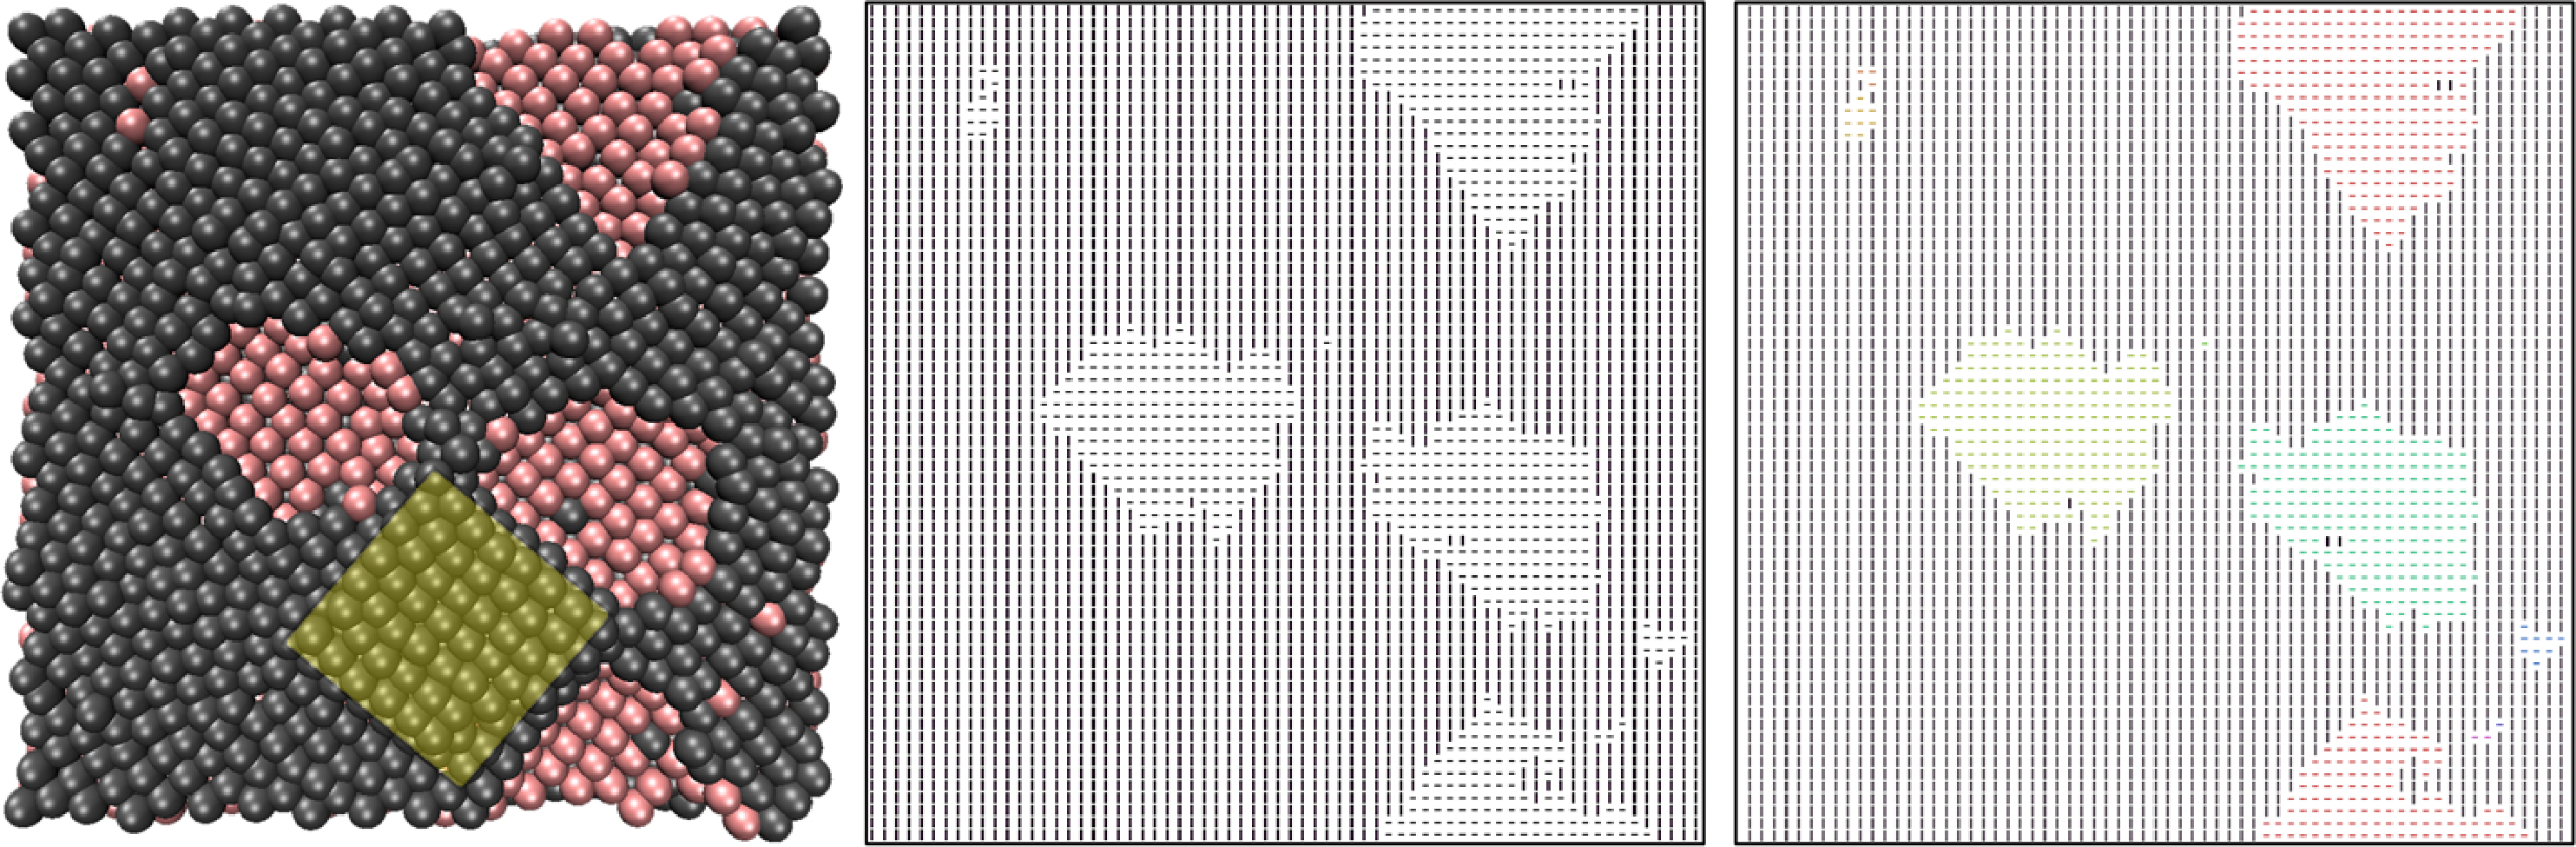
\includegraphics[width=\linewidth]{../figures/appD/grid_small.pdf}
  \caption{Analysis of the roughened surface to find surface domain sizes was
carried out by mapping the surface (left) onto 1-\AA\ spaced grid
points (center). Contiguous domains were identified and have been shown in
distinct colors (right), while the distribution of the domain areas was collected
over 1.5 ns time windows.}
\label{fig:surfaceGrid}
\end{figure}
\end{landscape}

As displayed in Figure \ref{fig:ds100Pt} \ce{CO} has a strong effect on the
size of the \ce{Pt} domains on the 100-1Pt-2Pd systems. When no \ce{CO} was
present, the size of the domains are essentially the size of the entire system,
the presence of two distinct peaks is due to the binning and averaging of both
top and bottom domain sizes that must be done to display the data in this
format. The 0.25 ML and 0.5 ML systems conversely, do show significant changes
over the 6 ns of data collection and the decrease in \ce{Pt} domain sizes is
matched, as expected by an increase in \ce{Pd} domain sizes as highlighted in
Figure \ref{fig:ds100Pd}. 

\begin{figure}
\centering
  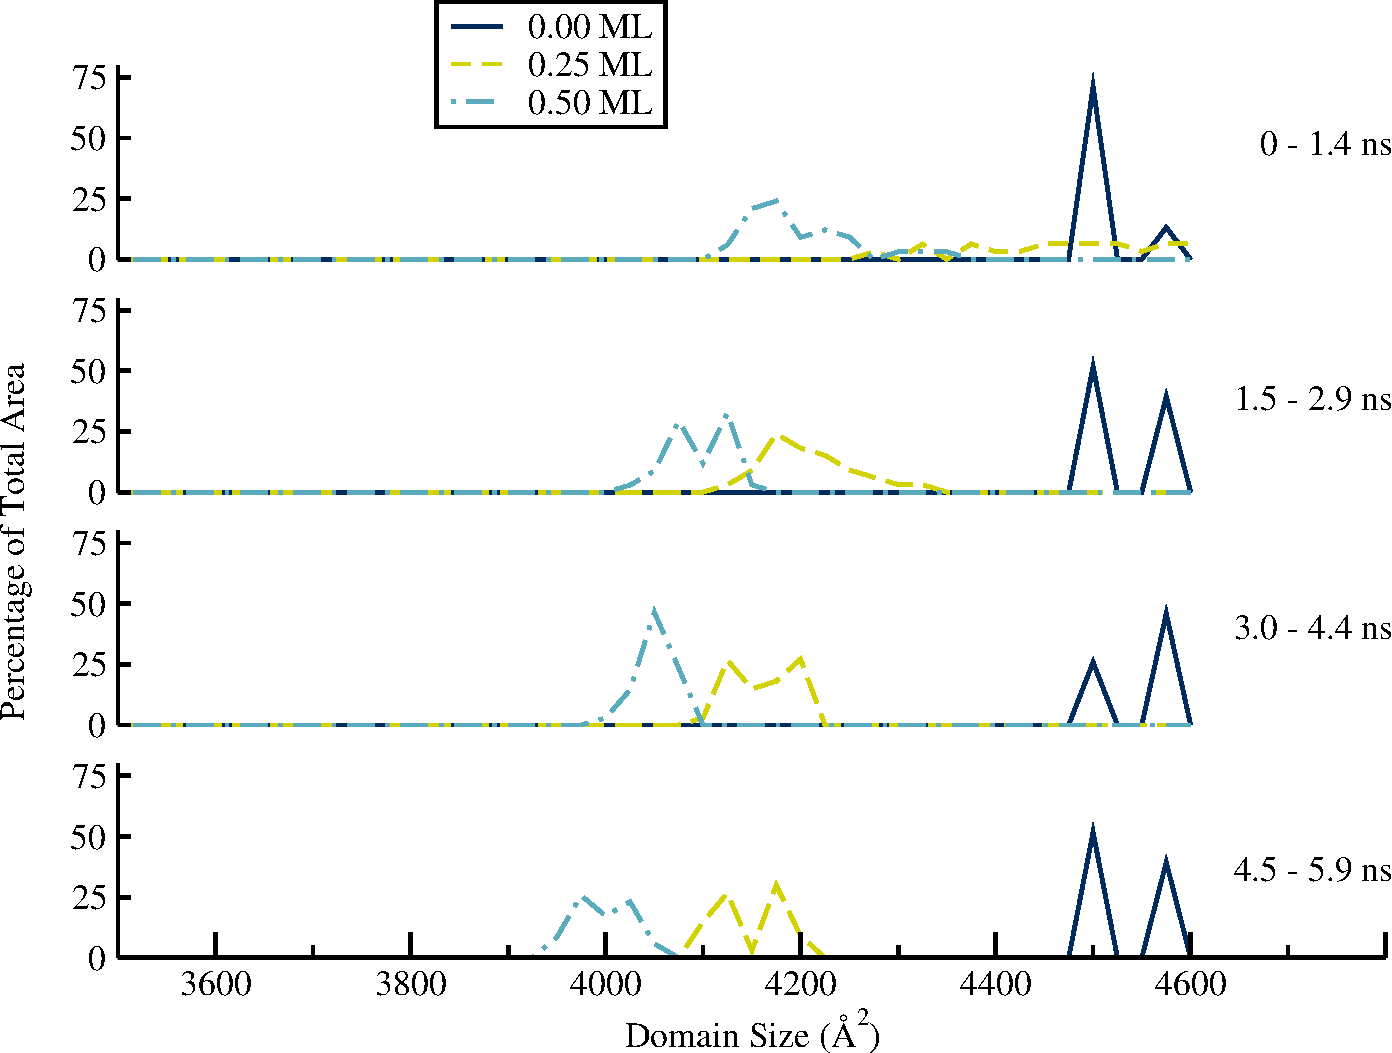
\includegraphics[width=\linewidth]{../figures/appD/ds_100_1Pt_2Pd_Pt.pdf}
  \caption{Distributions of Pt domain sizes at different CO coverages and at
different times after exposure to \ce{CO} for the 100-1\ce{Pt}-2\ce{Pd}
systems.}
\label{fig:ds100Pt}
\end{figure}


\begin{figure}
\centering
  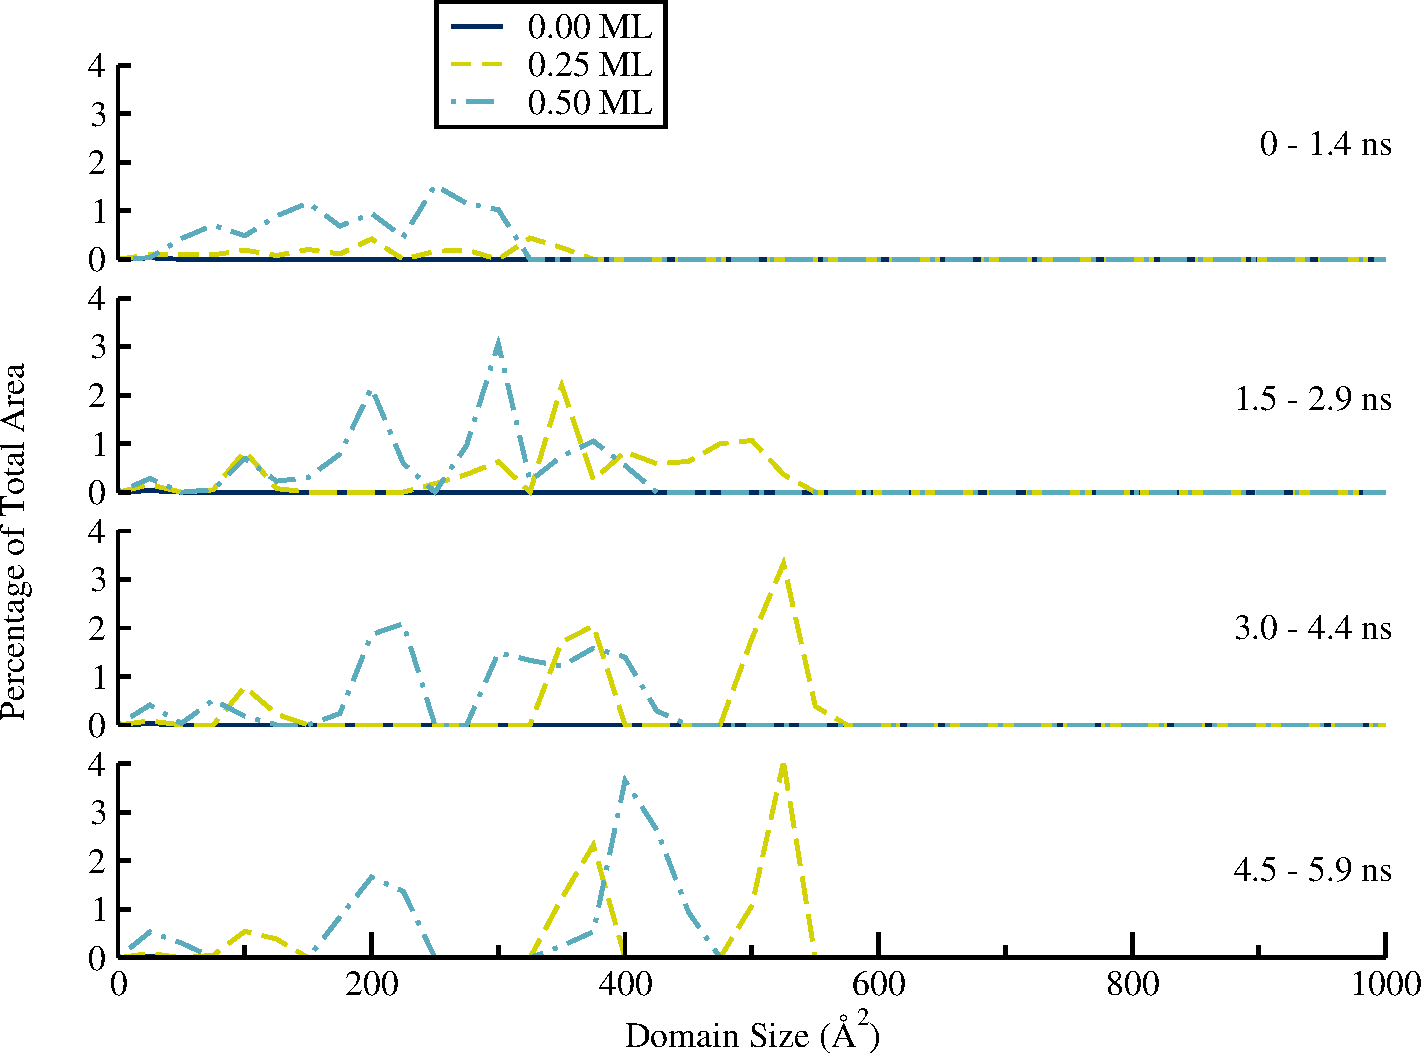
\includegraphics[width=\linewidth]{../figures/appD/ds_100_1Pt_2Pd_Pd.pdf}
  \caption{Distributions of Pd domain sizes at different CO coverages and at
different times after exposure to \ce{CO} for the 100-1\ce{Pt}-2\ce{Pd}
systems.}
\label{fig:ds100Pd}
\end{figure}

Similar to the inversion events, one of the driving forces for this
reconstruction is the stronger \ce{Pd\bond{-}CO} interaction which encourages
\ce{Pd} exposure at the alloy surface. However, the primary cause for these
domain formations is the inherent instability of the (100) overlayer when
compared to the lower energy (111) surface. However, as mentioned earlier and
highlighted in Figure \ref{fig:surfaceGrid}, despite the majority of the
surface \ce{Pt} collapsing to (111) domains, some of the \ce{Pt} atoms are
raised higher on the surface and retain the original (100) faceting.


\section{Summary}
The reconstruction that was observed on these systems was ultimately attributed
to the instability of the (100) surface facet rather than to any primarily
\ce{CO} induced effect. However, the presence of \ce{CO} did facilitate some of
this reconstruction as shown in the domain plots and inversion figures. Similar
to what was seen in Chapter \ref{chap:island}, the stronger \ce{Pd\bond{-}CO}
interaction coupled with the preference for \ce{Pt} to maximize nearest
neighbors provided the main driving forces for these reconstructions. The
presence of \ce{CO} also played a small role by weakening the metal-metal
bonds, speeding up many of these processes. Future simulations that ensure the
stability of the bare surfaces may be able to speak more clearly about the
effects of \ce{CO} on these systems.

